\chapter{ Sliding Mode controller}

The idea behind sliding mode is to force the states of a system to a so called sliding manifold and let it slide along this surface to the origin. When the states are on the surface the system show reduced order dynamics. To keep the system on the manifold a high frequency switching signal is needed. This can be obtained easily with a sign. As this would need to infinite fast switching , which cannot be realized, a boundary layer is introduced. This layer is achieved by using, instead of sign-function, another function like tanh.\\
To stabilize the error system of the robot arm the following sliding manifold is used:
\begin{gather*}
\mathbf{s} = \dot{\mathbf{e}} + \Lambda \mathbf{e}
\intertext{where:}
\begin{tabular}{>{$}l<{$} @{${}:{}$} l}
	\Lambda & diagonal matrix with time constants of the systems, when in sliding mode
\end{tabular}\nonumber
\end{gather*}

This system corresponds to a first order differential equation. To be stable the eigenvalues of this system needs to be negative. To control the robot the following control law is used:
\begin{gather*}
\tau_c = \hat{\mathbf{M}}\ddot{\mathbf{q}}_s + \hat{\mathbf{V}}_m \dot{\mathbf{q}}_s + \hat{\mathbf{g}} + \mathbf{K} sign(\mathbf{s})
\intertext{where:}
\begin{tabular}{>{$}l<{$} @{${}:{}$} l}
\hat{\mathbf{M}} & estimated inertia matrix\\
\hat{\mathbf{V}}_m & estimated centrifugal/coriolis matrix\\
\dot{\mathbf{q}}_s & $\Lambda \mathbf{e} + \mathbf{\dot{q}}_D$\\
\hat{\mathbf{g}} & estimated gravitation vector\\
\mathbf{K} & diagonal matrix with gains
\end{tabular}\nonumber
\end{gather*}

The parameter $\mathbf{K}$ is used to compensate for the unknown or unmodelled dynamics. The better the model is the smaller this parameter can be chosen.
For the simulation following parameter sets have been chosen: 
\begin{table}[h]
	\begin{center}
		\label{tab:smo}
		\begin{tabular}{lllll}
			&     &							 &Switching& According          \\
			$\lambda$ & $k$ &$\hat{\mathbf{g}}$&Function& Figure             \\
			\midrule
			10    & 20 &$0.75\mathbf{g}  $& sign(s)& \ref{fig:ch5_smo1} \\
			10    & 10 &$0.75\mathbf{g}  $& sign(s)& \ref{fig:ch5_smo2} \\
			25    & 20 &$0.75\mathbf{g}  $& sign(s)& \ref{fig:ch5_smo3} \\
			10    & 20 &$0\mathbf{g}  $& sign(s)& \ref{fig:ch5_smo4} \\
			10    & 30 &$0\mathbf{g}  $& sign(s)& \ref{fig:ch5_smo5} \\
			10    & 20 &$0\mathbf{g}  $& tanh(s)& \ref{fig:ch5_smo6} \\
			10    & 40 &$0\mathbf{g}  $& tanh(5s)& \ref{fig:ch5_smo7} \\
			\bottomrule
		\end{tabular}
		\caption{Controller parameters for simulations with sliding mode controller}
	\end{center}
\end{table}

In figure \ref{fig:ch5_smo1} it can be seen that the error converges after 0.5 to 1 second. The torques show the typical high frequency switching of the sliding mode control law.

\begin{figure}[]
	\centering
	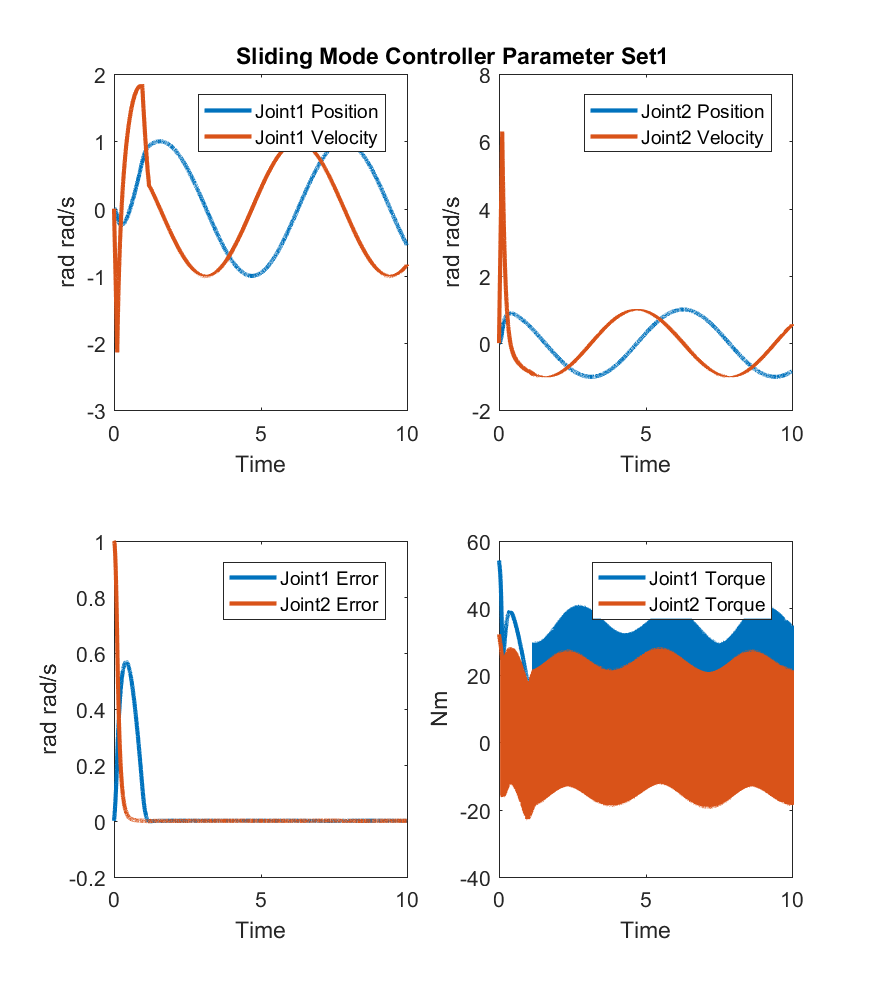
\includegraphics[width=0.85\textwidth]{pics/SlidingModeControllerParameterSet1.png}\\
	\caption{Sliding Mode Controller with $\lambda = 10, k=20,\hat{\mathbf{g}}=0.75\mathbf{g}$  }
	\label{fig:ch5_smo1}
\end{figure}

The simulation, which can be seen in figure \ref{fig:ch5_smo2}, has the linear gain of the switching function reduced, compared to the previous simulation. The result of the less aggressive controller, can be seen in the convergence time of the error, which is about twice the time compared to the previous parameter set. The values of the torques are also reduced, since the controller does react less aggressive.

\begin{figure}[]
	\centering
	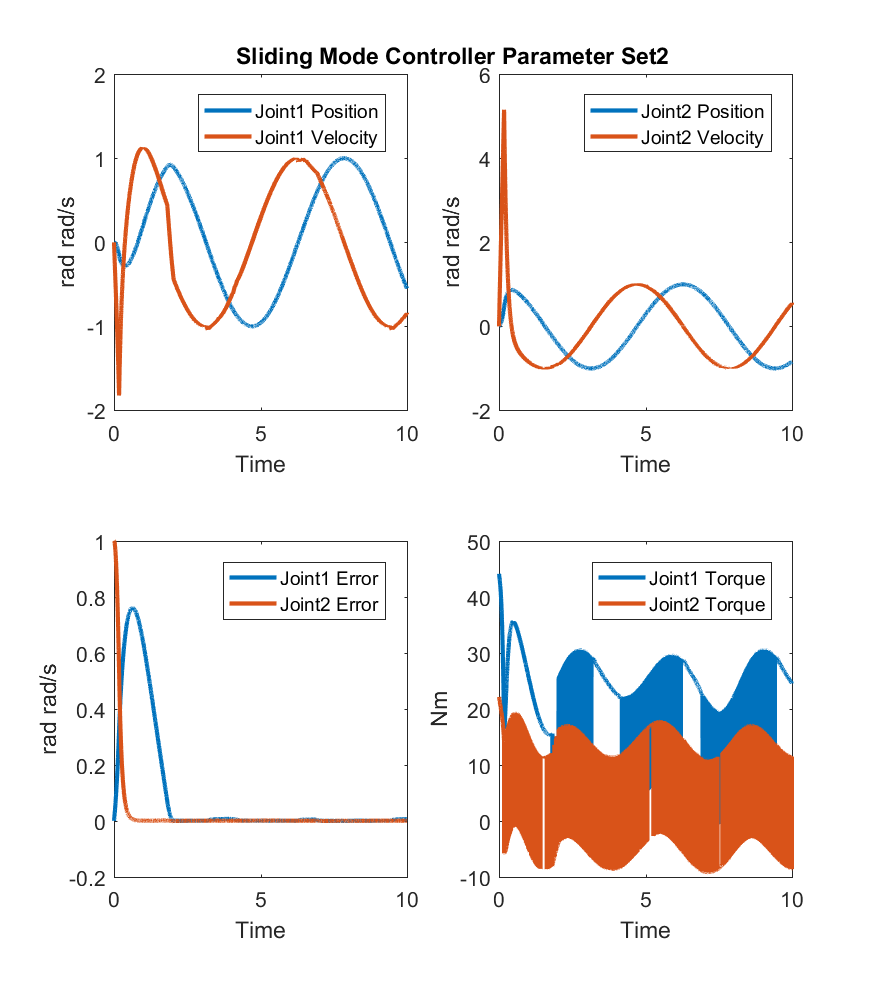
\includegraphics[width=0.85\textwidth]{pics/SlidingModeControllerParameterSet2.png}\\
	\caption{Sliding Mode Controller with $\lambda = 10, k=10,\hat{\mathbf{g}}=0.75\mathbf{g}$  }
	\label{fig:ch5_smo2}
\end{figure}

In figure \ref{fig:ch5_smo3} the simulation results are shown for a controller with increased values $\lambda$. The time to drive the error to zero is even more increased, compared to the previous simulations.
\begin{figure}[]
	\centering
	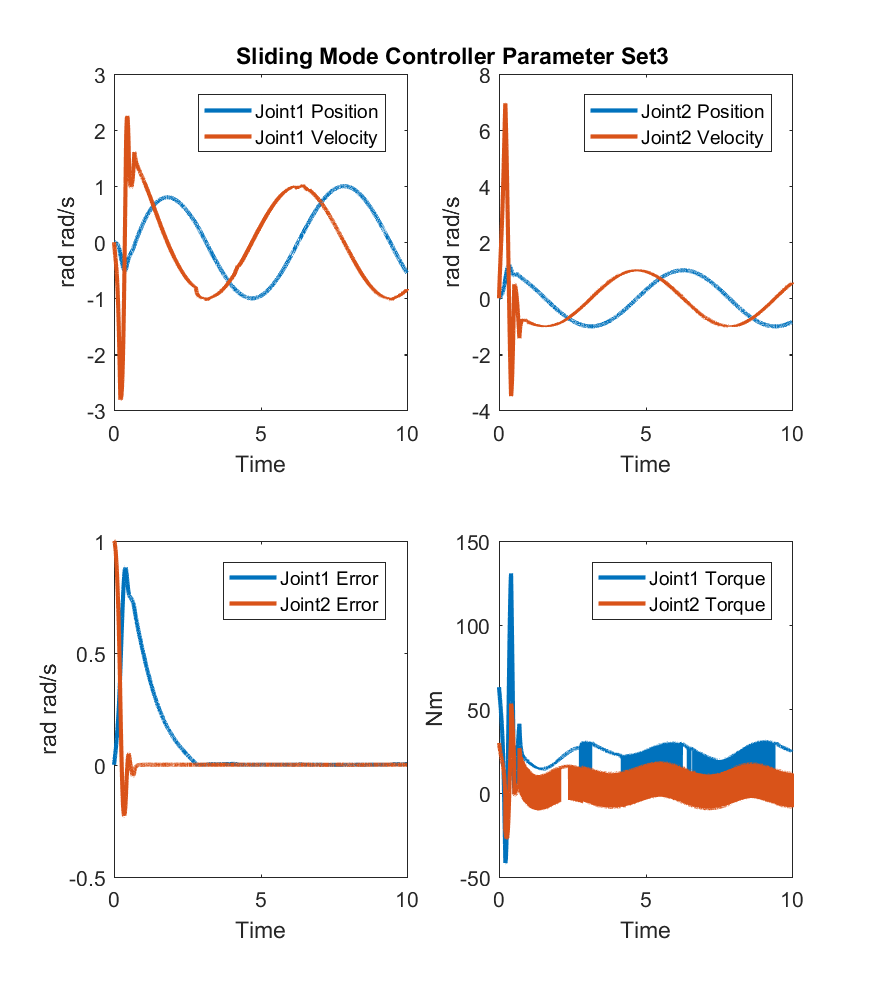
\includegraphics[width=0.85\textwidth]{pics/SlidingModeControllerParameterSet3.png}\\
	\caption{Sliding Mode Controller with $\lambda = 25, k=20,\hat{\mathbf{g}}=0.75\mathbf{g}$  }
	\label{fig:ch5_smo3}
\end{figure}

The next two simulation will show the results, if the gravitational component in the controller is ignored. The results in \ref{fig:ch5_smo4}  show that the error of the first joint does not converge anymore.
\begin{figure}[]
	\centering
	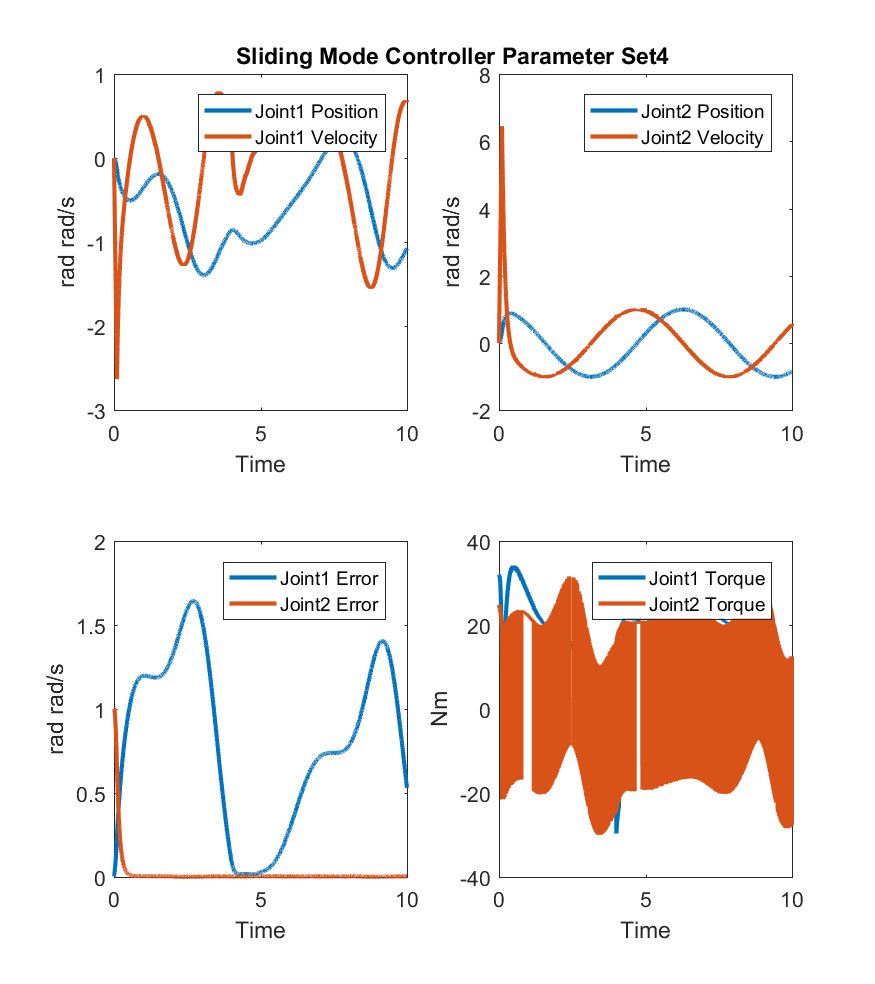
\includegraphics[width=0.85\textwidth]{pics/SlidingModeControllerParameterSet4.png}\\
	\caption{Sliding Mode Controller with $\lambda = 10, k=20,\hat{\mathbf{g}}=0\mathbf{g}$  }
	\label{fig:ch5_smo4}
\end{figure}

The next simulation has no gravitational term within the controller, although the parameters are tuned for an optimal behavior, which lead to $\lambda = 10, k=30 $. It can be seen that the controller is able to drive the error to zero after 3 seconds.

\begin{figure}[]
	\centering
	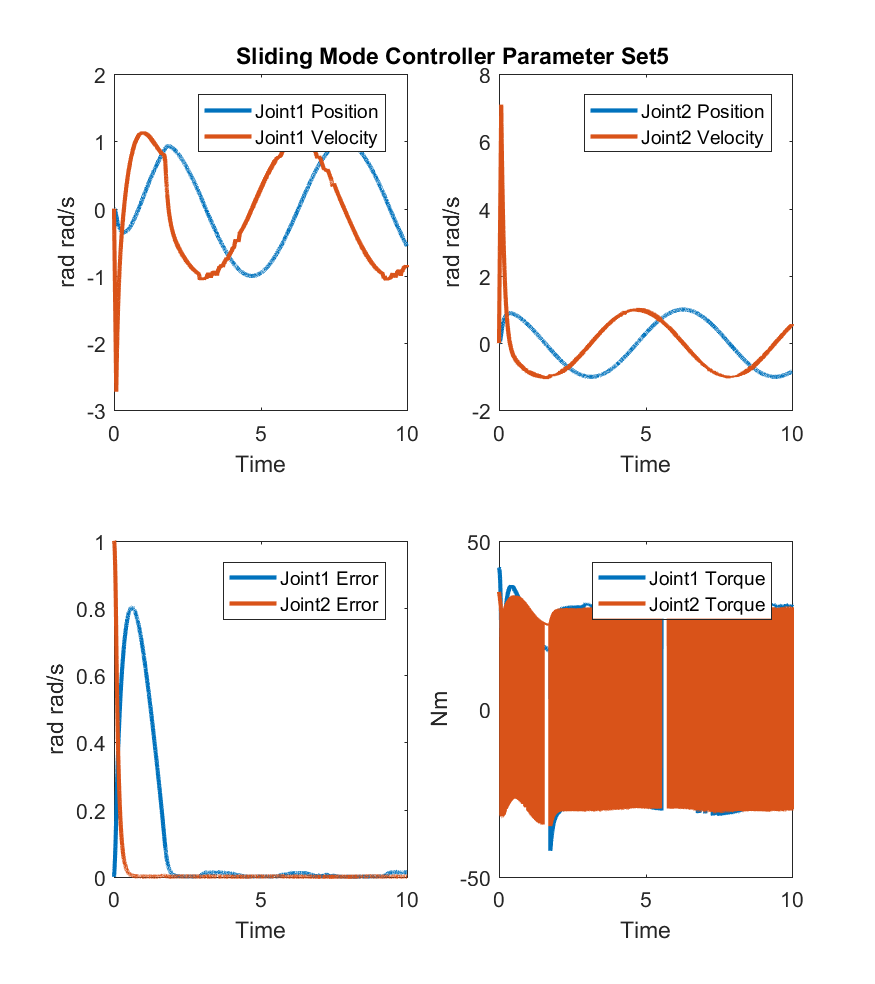
\includegraphics[width=0.85\textwidth]{pics/SlidingModeControllerParameterSet5.png}\\
	\caption{Sliding Mode Controller with $\lambda = 10, k=30,\hat{\mathbf{g}}=0\mathbf{g}$  }
	\label{fig:ch5_smo5}
\end{figure}

To check the influence of the switching function itself the following two simulations have been done with a non-ideal switching function, which introduces a boundary layer around the switching manifold. In this case the $tanh$ function has been used. In figure \ref{fig:ch5_smo6} it can be seen that the asymptotically stability of the error function did disappear and some oscillations can be seen. Therefore the torque itself does not show any high frequency switching anymore.
\begin{figure}[]
	\centering
	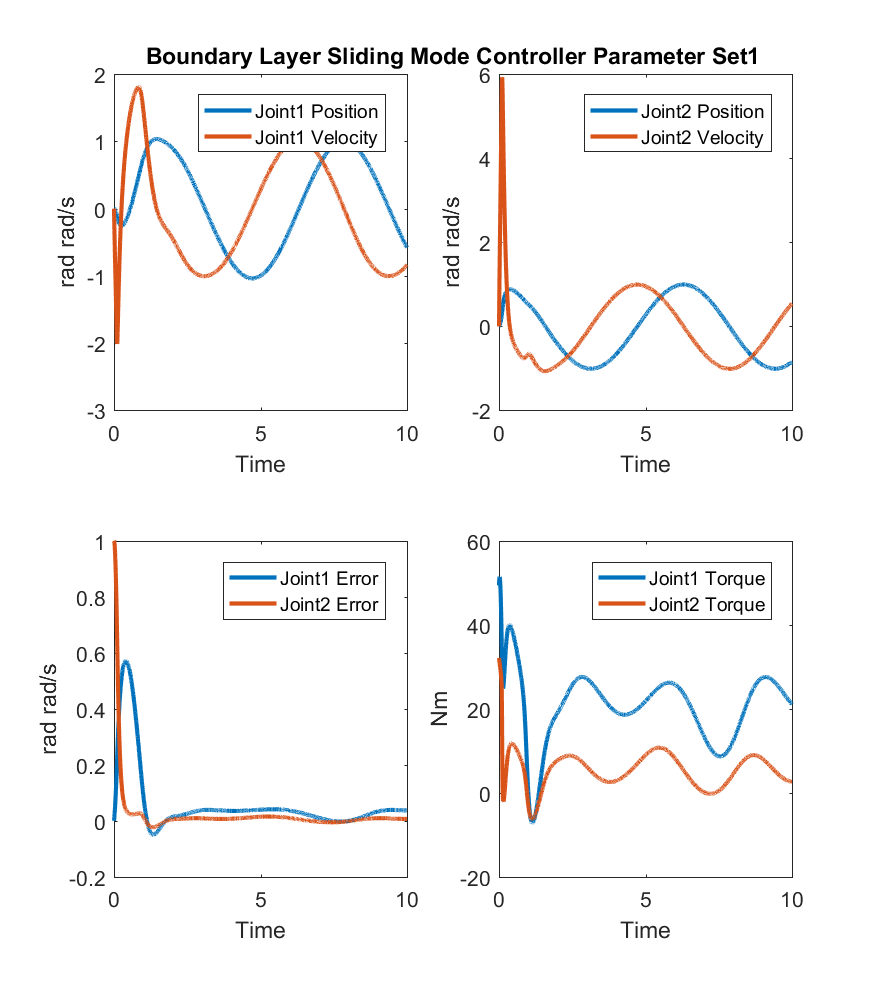
\includegraphics[width=0.85\textwidth]{pics/BoundaryLayerSlidingModeControllerParameterSet1.png}\\
	\caption{Boundary Layer Sliding Mode Controller with $\lambda = 10, k=20,\hat{\mathbf{g}}=0\mathbf{g}$  }
	\label{fig:ch5_smo6}
\end{figure}

In figure \ref{fig:ch5_smo7} the results can be seen with a more aggressive switching function by scaling the sliding function itself, this leads to a narrower boundary layer around the switching manifold. The torque values still do not show the high frequency switching, but the convergence of the error shows better behavior and is almost asymptotically stable.

\begin{figure}[]
	\centering
	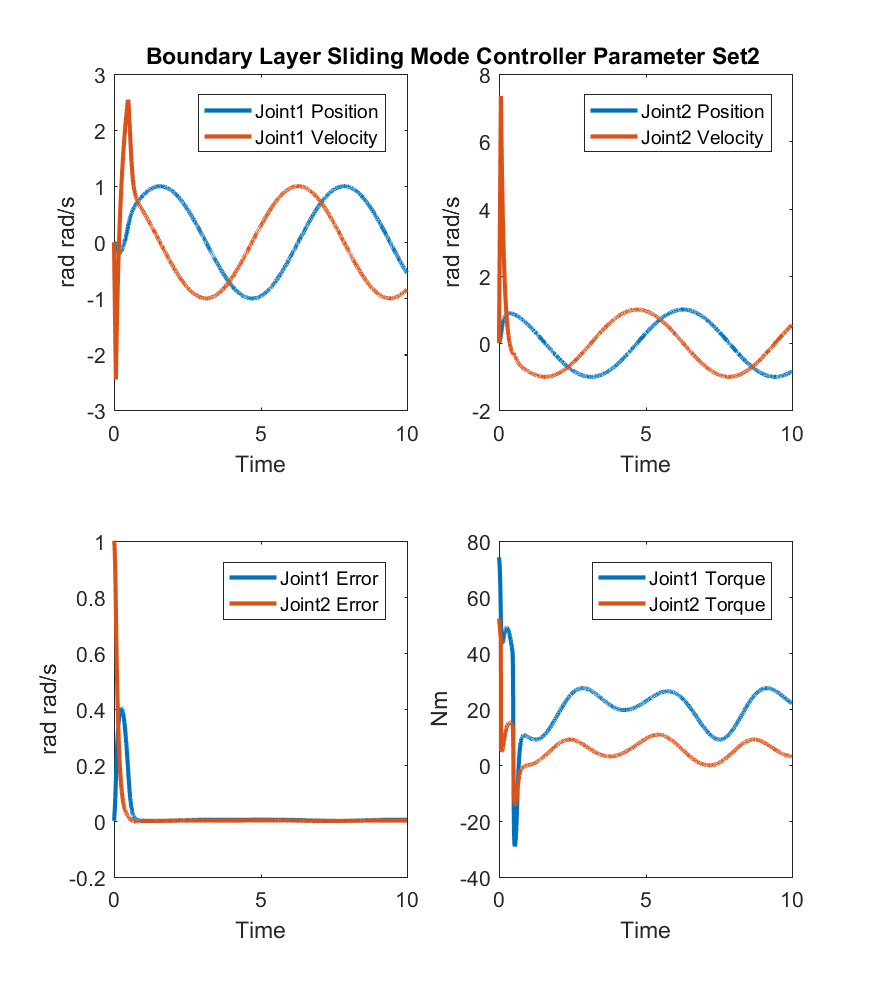
\includegraphics[width=0.85\textwidth]{pics/BoundaryLayerSlidingModeControllerParameterSet2.png}\\
	\caption{Boundary Layer Sliding Mode Controller with $\lambda = 10, k=40,\hat{\mathbf{g}}=0\mathbf{g}$  }
	\label{fig:ch5_smo7}
\end{figure}
